\chapter*{Proposition 31}



\begin{figure*}[ht]
    \begin{center}
    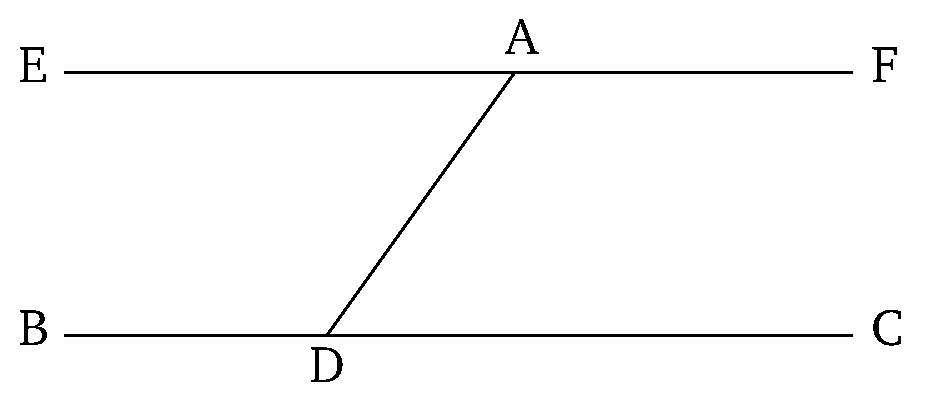
\includegraphics[width=0.5\linewidth]{figures/fig31e.eps}
    \label{fig:prop_31}
    \end{center}
\end{figure*}

To draw a straight-line parallel to a given straight-line, through a given
point.

Let $A$ be the given point, and $BC$ the given straight-line. So it is
required to draw a straight-line parallel to the straight-line $BC$, through
the point $A$.

Let the point $D$ have been taken a random  on $BC$, and let $AD$ have been
joined. And let (angle) $DAE$, equal to angle $ADC$,  have been constructed 
on the straight-line $DA$ at the point $A$ on it [Prop.~1.23]. And let the
straight-line $AF$ have been
produced in a straight-line with $EA$.

And since the straight-line $AD$, (in) falling across the two straight-lines
$BC$ and $EF$,  has made the alternate
angles $EAD$ and $ADC$ equal to one another, $EAF$ is thus parallel to $BC$
[Prop.~1.27].

Thus, the straight-line $EAF$ has been drawn parallel to the given straight-line $BC$, through the  given
point $A$. (Which is) the very thing it was required to do.


\section*{Commentary}

\begin{proposition}\label{proposition_31}\lean{Elements.Book1.proposition_31}\leanok
    If
\end{proposition}
\begin{proof}
    \uses{proposition_23,proposition_27}\leanok
\end{proof}
